\documentclass[a4paper, 12pt]{article}

%-----------------------------------------------------
%                      PACKAGES
% ----------------------------------------------------
\usepackage[T1]{fontenc}
\usepackage[latin9]{inputenc}
\usepackage{fancyhdr}
\usepackage{geometry}
\usepackage[colorlinks=true, linkcolor=blue,citecolor=blue, urlcolor=blue]{hyperref}
\usepackage{indentfirst}
\usepackage{graphicx}
\usepackage{float}
\usepackage{setspace}
\usepackage{amsmath}
\usepackage{amssymb}
\usepackage{multirow}
\usepackage[table,xcdraw]{xcolor}
\usepackage{colortbl}
\usepackage{tabularx,booktabs}
\usepackage{enumerate}
\usepackage{titlesec}
\usepackage{caption}
\usepackage{subcaption}
\usepackage{nicefrac, xfrac}
\usepackage{subfiles}
\usepackage{mathtools}
\usepackage{bm}
\usepackage{tikz}
\usepackage[mode=buildnew]{standalone}
\usepackage{systeme}
\usepackage{stmaryrd}
\usepackage{import}
\usepackage[english]{babel} 
\usepackage{times}
\usepackage{pgfplots}
\usepackage{makecell}
\usepackage{threeparttable}
\usepackage{ragged2e}
\usepackage{tocloft}
\usepackage{booktabs}
\usepackage[acronym]{glossaries}
\usepackage{pdfpages}
\usepackage{lipsum}
\usepackage{hyphenat} 
\usepackage{xspace}
\usepackage{abntex2cite}
\usepackage{pdflscape}
\usepackage{pythonhighlight}
\usepackage{listings}
\usepackage{makecell}

%-----------------------------------------------------
%               DOCUMENT SETTINGS
% ----------------------------------------------------
\geometry{a4paper,top=30mm,bottom=20mm,left=30mm,right=20mm}

\pgfplotsset{compat=1.17} 

\numberwithin{equation}{section}
\counterwithin{figure}{section}
\counterwithin{table}{section}
% \numberwithin{lstlisting}{section}

% Defining spaces between lines
\setstretch{1.5} 

\graphicspath{{Figures/}}

\tikzset{
	font={\fontsize{11pt}{12}\selectfont}}

\setcounter{secnumdepth}{4}
\setcounter{tocdepth}{4}

% defining the height of table cells
\renewcommand{\arraystretch}{1.4}

% defining the gradient, divergence, and curl operators
\newcommand{\grad}[1]{\nabla #1}
\renewcommand{\div}[1]{\nabla \cdot #1}
\newcommand{\curl}[1]{\nabla \times #1}

\def\textcite#1{\citeauthoronline{#1} \cite{#1}}
%-----------------------------------------------------
%              PRE TEXTUAL ELEMENTS
% ----------------------------------------------------
\newenvironment{epigrafe}{\newpage\mbox{}\vfill\hfill\begin{minipage}[t]{0.5\textwidth}}
{\end{minipage}\newpage}

%-----------------------------------------------------
%              PYTHON CODE SETTINGS
% ----------------------------------------------------
\definecolor{codegreen}{rgb}{0,0.6,0}
\definecolor{codegray}{rgb}{0.5,0.5,0.5}
\definecolor{codepurple}{rgb}{0.58,0,0.82}
\definecolor{backcolour}{rgb}{0.95,0.95,0.92}

\lstdefinestyle{mystyle}{
    backgroundcolor=\color{backcolour},   
    commentstyle=\color{codegreen},
    keywordstyle=\color{magenta},
    numberstyle=\tiny\color{codegray},
    stringstyle=\color{codepurple},
    basicstyle=\ttfamily\footnotesize,
    breakatwhitespace=false,         
    breaklines=true,                 
    captionpos=b,                    
    keepspaces=true,                 
    numbers=left,                    
    numbersep=5pt,                  
    showspaces=false,                
    showstringspaces=false,
    showtabs=false,                  
    tabsize=2
}

\lstset{style=mystyle}
%-----------------------------------------------------
%                     DOCUMENT 
% ----------------------------------------------------
\begin{document}
% ------- WORK INFORMATION -------
\author{Carlos Henrique Chama Puga }
\newcommand{\RA}{195416}

\title{List 3 \\ Decomposition and Storage of Matrices}
\newcommand{\theme}{Decomposition and Storage of Matrices}

\newcommand{\Uni}{{Universidade Estadual de Campinas}}
\newcommand{\Fac}{{Faculdade de Engenharia Civil, Arquitetura e Urbanismo}}

\newcommand{\advisor}{Porf. Dr. Philippe Devloo}
\newcommand{\coadvisor}{Dr. Giovane Avancini}

\newcommand*{\workyear}{2024}

\makeatletter

% ------- PRE TEXTUAL PAGES -------
% Could not find another way to remove the page number from the first pages
\fancypagestyle{plain}{
    \fancyhf{}% Limpa todos os campos
    \fancyfoot[C]{}%
    \renewcommand{\headrulewidth}{0pt}%
}

\pagestyle{plain}
\def\logos{
    \noindent
    \raisebox{-.5\height}{
\includegraphics[width=2.2cm]{Figures/logo-unicamp.pdf}}

    \vspace*{1.5cm}
    
    \noindent
    \begin{center} \large
        \MakeUppercase{\Uni}\\
        \Fac\\
    \end{center}
}

\def\openningpage{
  \logos
  \vskip 35mm
  \begin{center}
    \Large
      {\bf \@title}
  \end{center}
  \vskip 25mm
  \begin{flushright}
    \large
    {\textbf{Aluno:} \\ \@author - \RA}
    \vskip 10mm
    {{\bf{Docentes}}: \\
     \advisor \\
     \coadvisor}
  \end{flushright}
    \vfill
    \large
  \begin{center}
    Campinas\\\workyear
  \end{center}
}

\openningpage % Cover page

% Table of contents
\newpage
\tableofcontents 

% From here on, the page number is shown
% Chapter first page settings
\newpage
\fancypagestyle{plain}{
    \fancyhf{}% Limpa todos os campos
    \fancyhead[R]{\thepage}%
    \renewcommand{\headrulewidth}{0pt}%
}

\fancypagestyle{headings}{%
    \fancyhf{}% Limpa todos os campos
    \fancyhead[L]{\theme}% Nome do trabalho à esquerda
    \fancyhead[R]{\thepage}% Numero da página à direita
    \renewcommand{\headrulewidth}{1pt}%
}

% ------- CHAPTERS -------
\pagestyle{headings}
\section{Introduction} \label{sec:introduction}
It is possible to think of a matrix as a linear transformation applied to a vector. When the matrix is applied to a vector and the resulting vector is parallel to the original vector, this vector is said to be an eigenvector of the matrix so that 
\begin{equation}
    A\mathbf{v} = \lambda \mathbf{v},
    \label{eq:eigenvalue}
\end{equation}
in which $A$ is the matrix, $\mathbf{v}$ is the eigenvector, and $\lambda$ is the eigenvalue. 

Equation \eqref{eq:eigenvalue} can be rewritten as
\begin{equation}
    (A - \lambda I)\mathbf{v} = 0,
    \label{eq:eigenvalue_analytical}
\end{equation}
which means that, for any nonzero vector $\mathbf{v}$, Eq. \eqref{eq:eigenvalue_analytical} holds only if the determinant of the matrix $A - \lambda I$ is zero. In other words, matrix $A - \lambda I$ is singular. This is the characteristic equation of the matrix $A$ and can be used to find the eigenvalues of the matrix. 

Naturally, the eigenvalues of a matrix are the roots of the characteristic equation. However, a generalization of the characteristic equation is not always possible, and therefore, its analytical solution is not always feasible. 

The Power Method is an iterative method that can be used to find the most prominent eigenvalue of a matrix. The method is simple to implement and can be used to find both the eigenvalue and the eigenvector of the matrix. 

For a given vector $\mathbf{y}$ linearly independent of $\mathbf{v}$, it is possible to write
\begin{equation}
    \mathbf{y} = \sum_{i=1}^{n}\beta_i\mathbf{v}_i,
    \label{eq:linear_combination}
\end{equation}
in which $\mathbf{v}_i$ are the eigenvectors of the matrix $A$. 

Multiplying Eq. \eqref{eq:linear_combination} by $A^k$ yields
\begin{equation}
    A^k\mathbf{y} = \sum_{i=1}^{n}\beta_i\lambda_i^k\mathbf{v}_i,
    \label{eq:eigenvalue_power}
\end{equation}
and factoring Eq. \eqref{eq:eigenvalue_power} by $\lambda_1^k$ gives
\begin{equation}
    {A^k\mathbf{y}} = {\lambda_1^k}\sum_{i=1}^{n}\beta_i\left(\frac{\lambda_i}{\lambda_1}\right)^k\mathbf{v}_i.
    \label{eq:eigenvalue_power_factor}
\end{equation}

Since $\lambda_1$ is the most prominent eigenvalue, the term $\left(\frac{\lambda_i}{\lambda_1}\right)^k$ tends to zero for $i \neq 1$. Therefore, the term $\sum_{i=1}^{n}\beta_i\left(\frac{\lambda_i}{\lambda_1}\right)^k\mathbf{v}_i$ tends to $\beta_1\lambda_1^k\mathbf{v}_1$ as $k$ tends to infinity. 

This is the main idea behind the Power Method. The method starts with an initial guess $\mathbf{v}_0$. The matrix $A$ is multiplied by $\mathbf{v}_0$ to find the next eigenvector
\begin{equation}
    \mathbf{y} = A\mathbf{v}_{i-1},
    \label{eq:y}
\end{equation}
the norm of the result is calculated and considered the new eigenvalue
\begin{equation}
    \lambda_i = \left\|\mathbf{y}\right\|,
\end{equation}
the new eigenvector is the previous result divided by the new eigenvalue
\begin{equation}
    \mathbf{v}_i = \frac{\mathbf{y}}{\lambda_i},
\end{equation}

This process is repeated until the error between the current and previous eigenvalues is smaller than a given precision. Since Eq. \eqref{eq:y} is performed at each iteration, the limit when $k$ tends to infinity is approached.

The matrix $A$ can also be decomposed into the matrices $\Lambda$ and $Q$ so that
\begin{equation}
    A = Q\Lambda Q^{-1},
    \label{eq:decomposition}
\end{equation}
where $\Lambda$ is a diagonal matrix with the eigenvalues of $A$ 
\begin{equation*}
    \Lambda = \begin{bmatrix}
        \lambda_1 & 0 & \cdots & 0 \\
        0 & \lambda_2 & \cdots & 0 \\
        \vdots & \vdots & \ddots & \vdots \\
        0 & 0 & \cdots & \lambda_n
    \end{bmatrix},
\end{equation*}
and $Q$ is a matrix with the eigenvectors of $A$
\begin{equation*}
    Q = \begin{bmatrix}
        \mathbf{v}_1 & \mathbf{v}_2 & \cdots & \mathbf{v}_n
    \end{bmatrix}.
\end{equation*}

In the next sections, the power method is implemented and the results are discussed. The following bibliography is referred to in this work: \cite{de2000metodos,burden1997numerical}.
\section{The Full Matrix Class}\label{sec:fullmatrix}
The FullMatrix class is developed to store and manipulate dense matrices. The class is implemented in Python and has as methods the basic constructor, the SetDecompositionMethod, RankOneUpdtade, Fill\_L, Fill\_U, Fill\_D, Pivot, Lu\_Decompostion, LDLT\_Decompostion, FindInverse, and Decompose. Each one of these methods is described in the following sections. 

The main goal of this class is to decompose a given matrix and compare not only if the decomposition could be done, but whether the decomposition is correct. The inverse of the matrix is calculated as a way to check the accuracy of the code. 
\subsection{Class Implementation} \label{sec:fullmatrix_implementation}
The class FullMatrix has the following attributes: 
\begin{lstlisting}[language=Python, caption={FullMatrix constructor.}, label={code:main}] 
@dataclass
class FullMatrix:
    tolerance: ClassVar[float] = 1e-11 # Tolerance for the decomposition

    A: np.array # Matrix
    pivoting: bool = False # Pivoting flag
    diagonal: bool = False # Diagonal flag
    decomposition_type: str = None # Decomposition type
    size: int = field(init=False) # Matrix size

    A_Decomposed: np.array = field(init=False) # Decomposed matrix
    L: np.array = field(init=False) # Lower matrix
    U: np.array = field(init=False) # Upper matrix
    D: np.array = field(init=False) # Diagonal matrix

    detA: float = field(init=False) # Determinant of A
    inverseA: np.array = field(init=False) # Inverse of A
    decomposed_inverse: np.array = field(init=False) # Inverse of A by decomposition

    permuted_rows: list = field(default_factory=list) # permuted rows
    permuted_cols: list = field(default_factory=list) # permuted columns

    A_Memory: int = field(init=False, default=0) # Memory usage of the matrix
\end{lstlisting}

Among the attributes, the most important ones are the matrix A, which storages the full matrix itself, the decomposition\_type, responsible for setting which type of decomposition will be used, A\_Decomposed, which stores the decomposed matrix, L, D, and U, which stores the lower, diagonal and upper decomposed matrices. Notice that regardless of the method, a diagonal matrix is always created but initialized as an Identity matrix. 

One cites as well the permutation\_rows and permutations\_cols attributes, which are used during the pivoting process. The A\_Memory attribute stores how much memory is used by the matrix and will be used for further comparisons between full and sparse matrices. 

The first method that is implemented is the Decompose method. This function performs the decomposition depending on the decomposition\_type attribute. The method is shown in Listing \ref{code:decompose}.
\begin{lstlisting}[language=Python, caption={Decompose method.}, label={code:decompose}]
def Decompose(self)->None:
    if self.CheckSingularity():
        raise Exception("Singular matrix")
    
    if not self.Check_Symmetry() and (self.decomposition_type == "LDLt"):
        raise Exception("Matrix not symmetric.")
    
    if self.pivoting:
        self.Pivot_Decomposition()

    elif self.decomposition_type == "LU":
        self.LU_Decomposition()

    elif self.decomposition_type == "LDLt":
        self.LDLt_Decomposition()

    else:
        text = f"The '{self.decomposition_type}' decomposition is not valid. Please choose one of the following: LU, LDLt "
        raise Exception(text)
\end{lstlisting}
In line 2, the method checks if the matrix is singular. If it is, an exception is raised since the decomposition cannot be done. Line 5 checks if the matrix is symmetric once the LDLt is only valid for symmetric matrices. If the matrix is not symmetric, an exception is raised. Finally, in line 8 the decomposition is performed according to the decomposition\_type attribute. If the decompostion type does not match any of the implemented methods, an exception is raised.

Due to their simplicity, LU\_Decompostion and LDLt\_Decompostion methods are not shown first. Concepts like RankOneUpdate and Fill\_L, Fill\_U, and Fill\_D are explained in the following sections. Then, the Pivot\_Decomposition method is commented. 

From the implementation standpoint, both LU and LDLt implementations are alike. Basically what is done is to subtract each equation from the submatrix below it, updating the matrix using the rank one update method. Code \ref{code:decompostion} shows the main idea of the decomposition methods.
\begin{lstlisting}[language=Python, caption={Decomposition method.}, label={code:decompostion}]
def LU_Decomposition(self)->None:
    self.RankOneUpdate()
    self.Fill_L()
    self.Fill_U()

def LDLt_Decomposition(self)->None:
    self.RankOneUpdate()
    self.Fill_L()
    self.Fill_D()
    self.U = self.L.T
\end{lstlisting}

Comparing both methods in Code \ref{code:decompostion}, one realizes that the class is implemented in a manner to avoid code repetition. The only difference is that the LDLt method fills the diagonal matrix D with the Fill\_D method and the U matrix is the transpose of the L matrix. Code \ref{code:rankoneupdate} shows the RankOneUpdate method adapted for both LU and LDLt decompositions.
\begin{lstlisting}[language=Python, caption={RankOneUpdate method.}, label={code:rankoneupdate}]
def RankOneUpdate(self)->None:
    for i in range(self.size):
        matii_correction = 1.0

        if (abs(self.A_Decomposed[i, i]) < self.tolerance):
            raise Exception("Null Pivot")

        if self.decomposition_type in == "LDLt":
            matii_correction = self.A_Decomposed[i, i]
            self.A_Decomposed[i, i+1::] /= self.A_Decomposed[i, i]

        self.A_Decomposed[i+1::, i] /= self.A_Decomposed[i, i]
        self.A_Decomposed[i+1::, i+1::] -= OUTER(self.A_Decomposed[i+1::, i], self.A_Decomposed[i, i+1::]) * matii_correction
\end{lstlisting}

The main difference between the Lu and LDLt rank one update is that, for the former only the column below the pivot is updated, while for the latter both row and column are updated. Due to this fact, for LDLt it is necessary to correct the value of the submatrix formed by the outer product of the row and column vectors (matii\_correction = A\_Decomposed[i, i], rather than 1).

Line 5 raises the issue when the pivot is null. Since the row and column are divided by it, the rank one update is not possible. To overcome this problem, the Pivot method is implemented. The Pivot\_Decompostion method is shown in Code \ref{code:pivotdecomp}.
\begin{lstlisting}[language=Python, caption={Pivot method.}, label={code:pivotdecomp}]
def Pivot_Decomposition(self)->None:
    for index in range(self.size - 1):
        self.Pivot(index)
        
        if (abs(self.A_Decomposed[index, index]) < self.tolerance):
            raise Exception("Null Pivot.")

        matii_correction = 1.0

        if self.decomposition_type == "LDLt":
            matii_correction = self.A_Decomposed[index, index]
            self.A_Decomposed[index, index+1::] /= self.A_Decomposed[index, index]

        self.A_Decomposed[index+1::, index] /= self.A_Decomposed[index, index]
        self.A_Decomposed[index+1::, index+1::] -= OUTER(self.A_Decomposed[index+1::, index], self.A_Decomposed[index, index+1::]) * matii_correction

    self.Fill_L()
    if self.decomposition_type == "LU":
        self.Fill_U()

    elif self.decomposition_type == "LDLt":
        self.Fill_D()
        self.U = self.L.T

    self.permuted_rows = self.PermutationMatrix(self.permuted_rows)
    self.permuted_cols = self.PermutationMatrix(self.permuted_cols, rows=False)
\end{lstlisting}

Notice that the rank one update is now evaluated in each iteration to find the pivot, instead of from start to beginning. This ensures that the pivoting will guarantee the convergence of the decomposition method. Line 6 shows the Pivot method being called (see Code \ref{code:pivot}). Lines 11 - 19 evaluate the rank one updated. Lines 20 - 26 fill the matrices L, D, and U. Finally, lines 28 and 29 create the permutation matrices for rows and columns. 
\begin{lstlisting}[language=Python, caption={Pivot method.}, label={code:pivot}]
def Pivot(self, index:int)->None:
    rows = [i for i in range(self.size)]
    cols = [i for i in range(self.size)]

    submatrix = self.A_Decomposed[index::, index::].copy()

    row_max, col_max = self.FindMaxRowAndCol(submatrix)
    row_max += index
    col_max += index

    rows, cols = self.UpdatedPermutationVector(rows, cols, row_max, col_max, index)

    perm_row = self.PermutationMatrix(rows)
    perm_col = self.PermutationMatrix(cols, rows=False)

    self.A_Decomposed = perm_row @ self.A_Decomposed @ perm_col
\end{lstlisting}
The pivot method is simple and consists of finding the maximum value in the submatrix below the pivot to permute the rows and columns. Special attention is paid to the LDLt decomposition in which the maximum value is found in the diagonal to maintain the symmetry of the matrix. A flag, diagonal, can also be set to force the LU decomposition to look for the maximum value in the diagonal as well.

The Fill\_L, Fill\_U, and Fill\_D methods are simple and are shown in Code \ref{code:fill}.
\begin{lstlisting}[language=Python, caption={Fill\_L, Fill\_U, and Fill\_D methods.}, label={code:fill}]
def Fill_L(self)->None:
    for i in range(diagonal_aux1, self.size):
        for j in range(i + diagonal_aux2):
            self.L[i, j] = self.A_Decomposed[i, j]

def Fill_U(self)->None:
    diagonal_aux1 = 0 if self.decomposition_type == "LU" else 1 # row used to start filling the matrix
    diagonal_aux2 = 1 if self.decomposition_type == "LU" else 0 # column used to start filling the matrix

    for j in range(diagonal_aux1, self.size):
        for i in range(j + diagonal_aux2):
            self.U[i, j] = self.A_Decomposed[i, j]

def Fill_D(self)->None:
    for i in range(self.size):
        self.D[i, i] = self.A_Decomposed[i, i]
\end{lstlisting}

Lastly, the FindInverse method, used to compare the inverse of the original matrix and the one obtained after the decomposition, is shown in Code \ref{code:inverse}.
\begin{lstlisting}[language=Python, caption={FindInverse method.}, label={code:inverse}]
def FindInverse(self)->None:
    if self.pivoting:
        self.decomposed_inverse = self.permuted_rows.T @ INVERSE(self.U) @ INVERSE(self.D) @ INVERSE(self.L) @ self.permuted_cols.T
    
    elif self.decomposition_type in ["LU", "LDLt"]:
        self.decomposed_inverse = INVERSE(self.U) @ INVERSE(self.D) @ INVERSE(self.L)
    
    else:
        raise Exception(f"The '{self.decomposition_type}' decomposition is not valid.")
\end{lstlisting}

Equations \eqref{eq:inverse_pivot} and \eqref{eq:inverse} display the inverse of the matrix with and without the need for pivoting
\begin{equation}
    \label{eq:inverse_pivot}
    pR^T.U^{-1}.D^{-1}.L^{-1}.pC^T,    
\end{equation}
\begin{equation}
    \label{eq:inverse}
    U^{-1}.D^{-1}.L^{-1}
\end{equation}
where $pR$ and $pC$ are the permutation matrices for rows and columns, respectively, and the $.$ operator indicates the matrix multiplication.

The following sections show the results for decompositions LU and LDLt and the comparison between their inverse and the original matrix. The evaluation of the determinant shows that the matrix is not singular, i.e., the determinant is different from zero. Being so, the decomposition can be done. However, due to a zero on the diagonal, pivoting is necessary to avoid division by zero. Matrix A and its inverse are given in figues \ref{fig:matrix_A} and \ref{fig:matrix_A_inverse}.
\begin{figure}[H]
    \centering 
    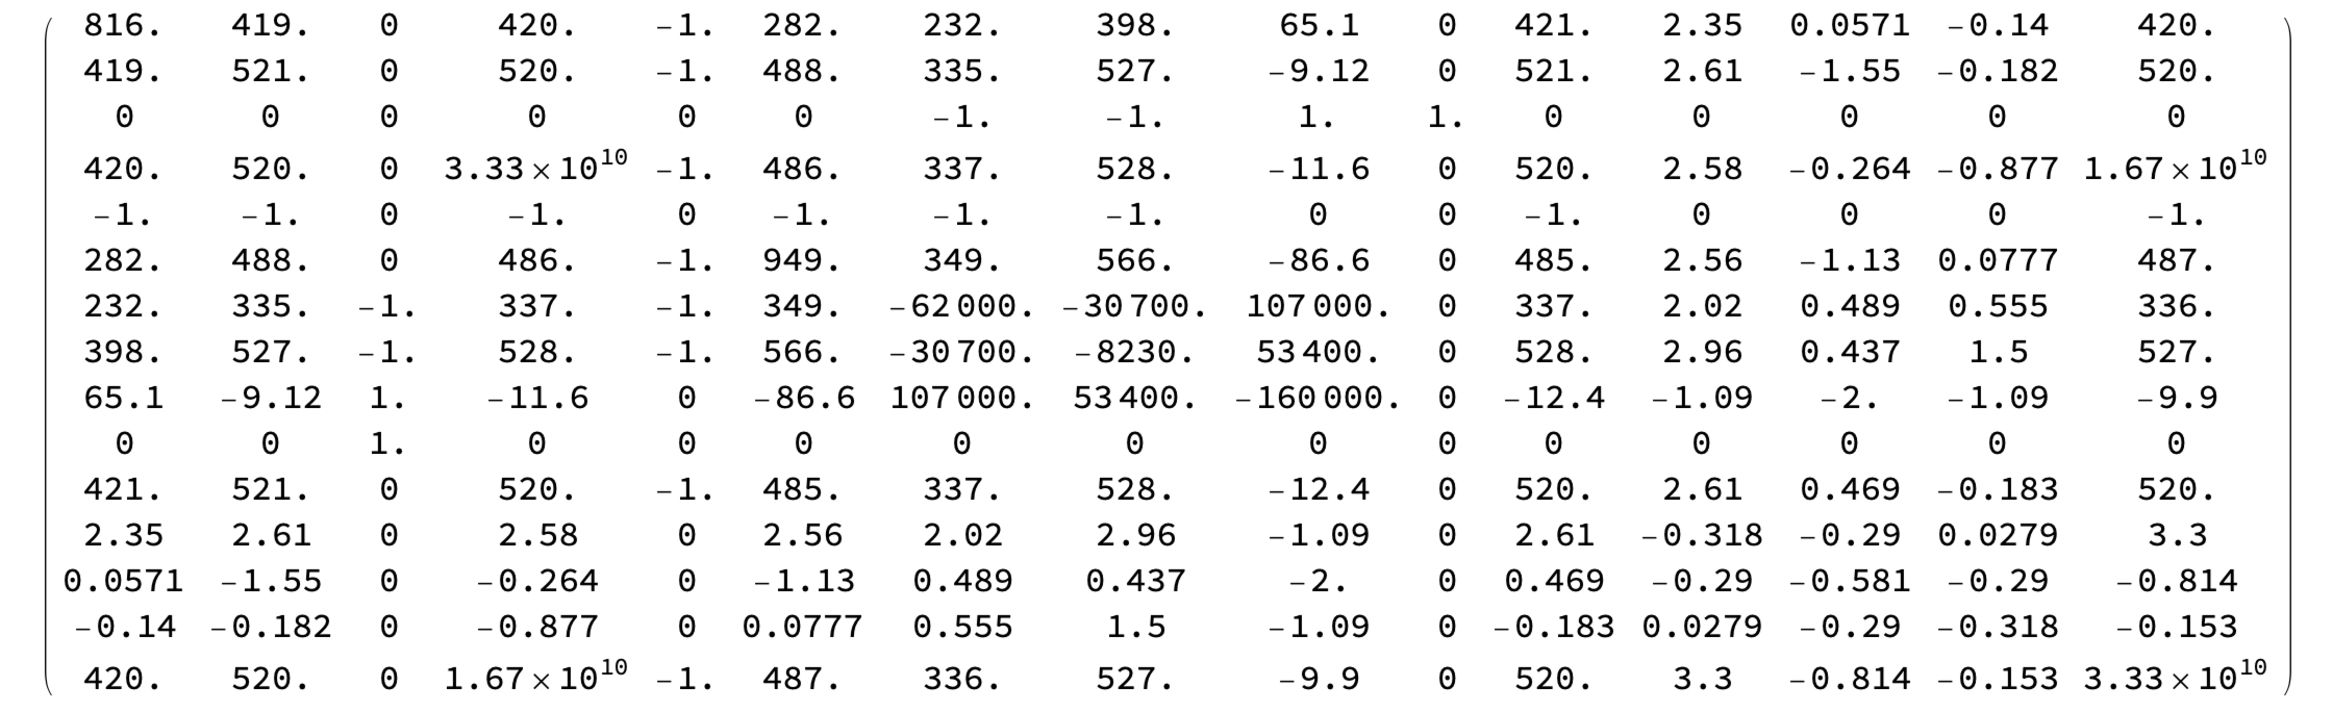
\includegraphics[width=1\textwidth]{MatrixA.pdf}
    \caption{Matrix A.}
    \label{fig:matrix_A}
\end{figure}
\begin{figure}[H]
    \centering 
    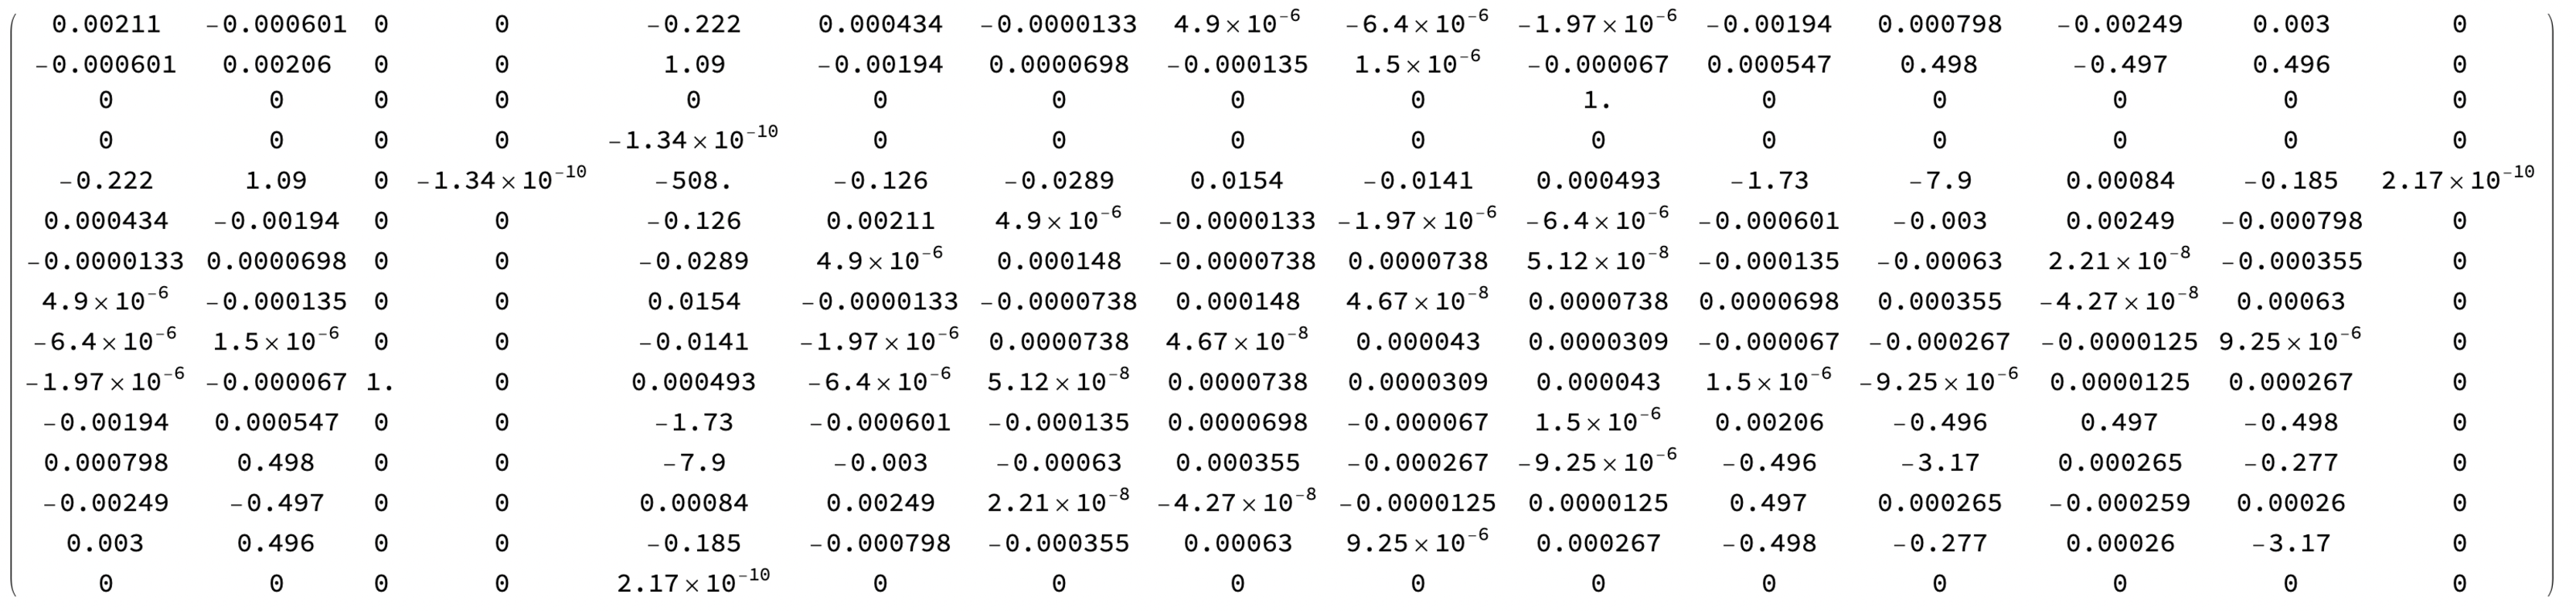
\includegraphics[width=1\textwidth]{InverseA.pdf}
    \caption{Matrix A inverse.}
    \label{fig:matrix_A_inverse}
\end{figure}

Appendix \ref{sec:mainFunction} shows the code for the main function, used throughout this report.

\subsection{Matrix LU Decomposition} \label{sec:lu}
LU decomposition follows the methods aforementioned. Results for the decomposition can be read in the .txt written by the Python algorithm. The main results for L, U and the error between the original matrix inverse and the decomposed matrix inverse are shown in figures \ref{fig:lu_L} - \ref{fig:lu_inverse_error}. 
\begin{figure}[H]
    \centering
    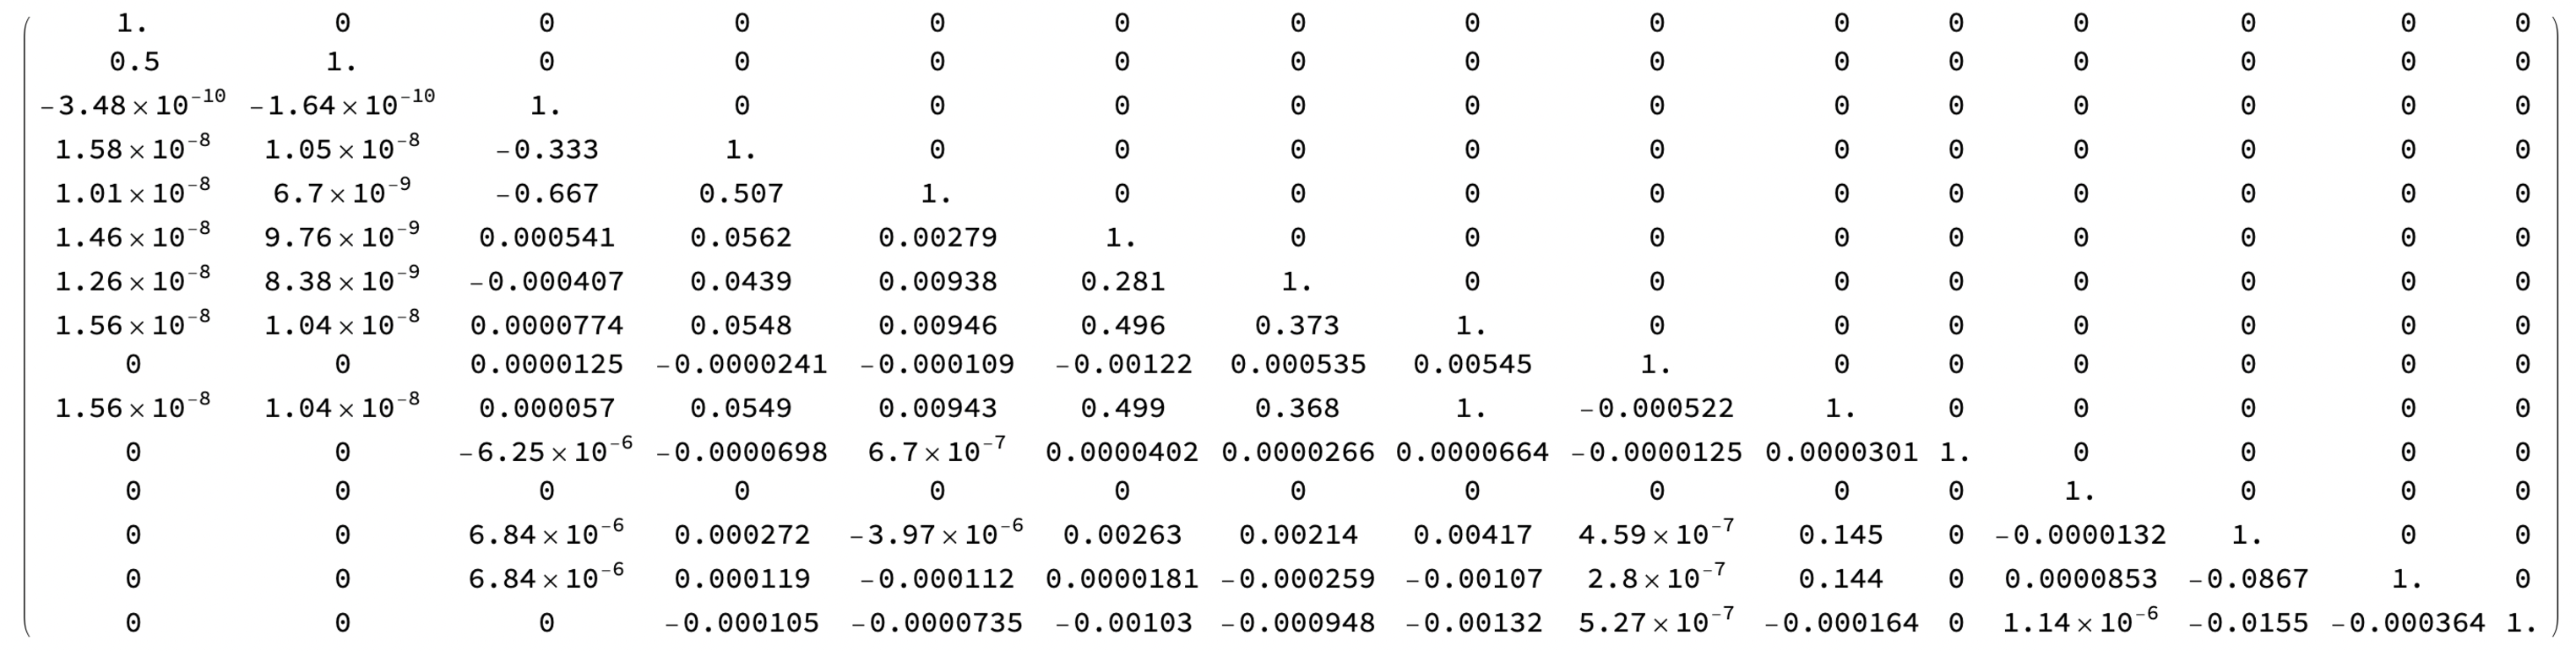
\includegraphics[width=1\textwidth]{L_lu.pdf}
    \caption{Matrix L (LU decomposition).}
    \label{fig:lu_L}
\end{figure}
\begin{figure}[H]
    \centering
    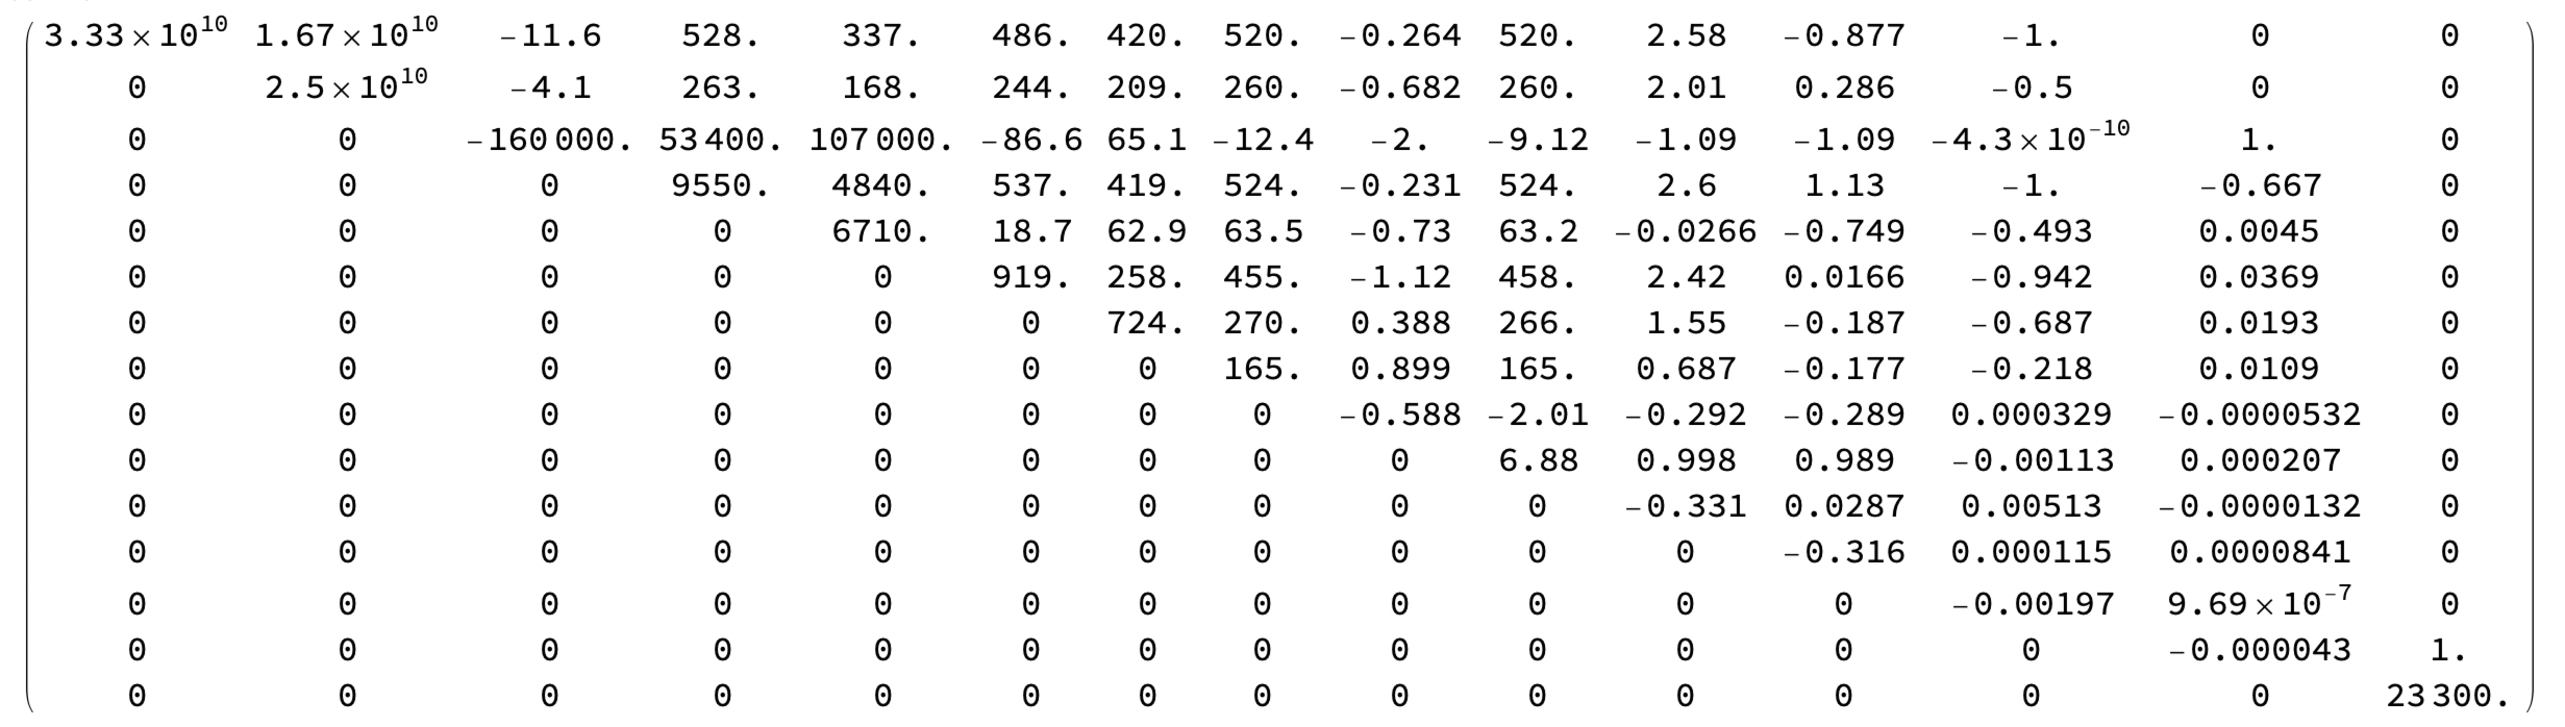
\includegraphics[width=1\textwidth]{U_lu.pdf}
    \caption{Matrix U (LU decomposition).}
    \label{fig:lu_inverse_error}
\end{figure}
\begin{figure}[H]
    \centering
    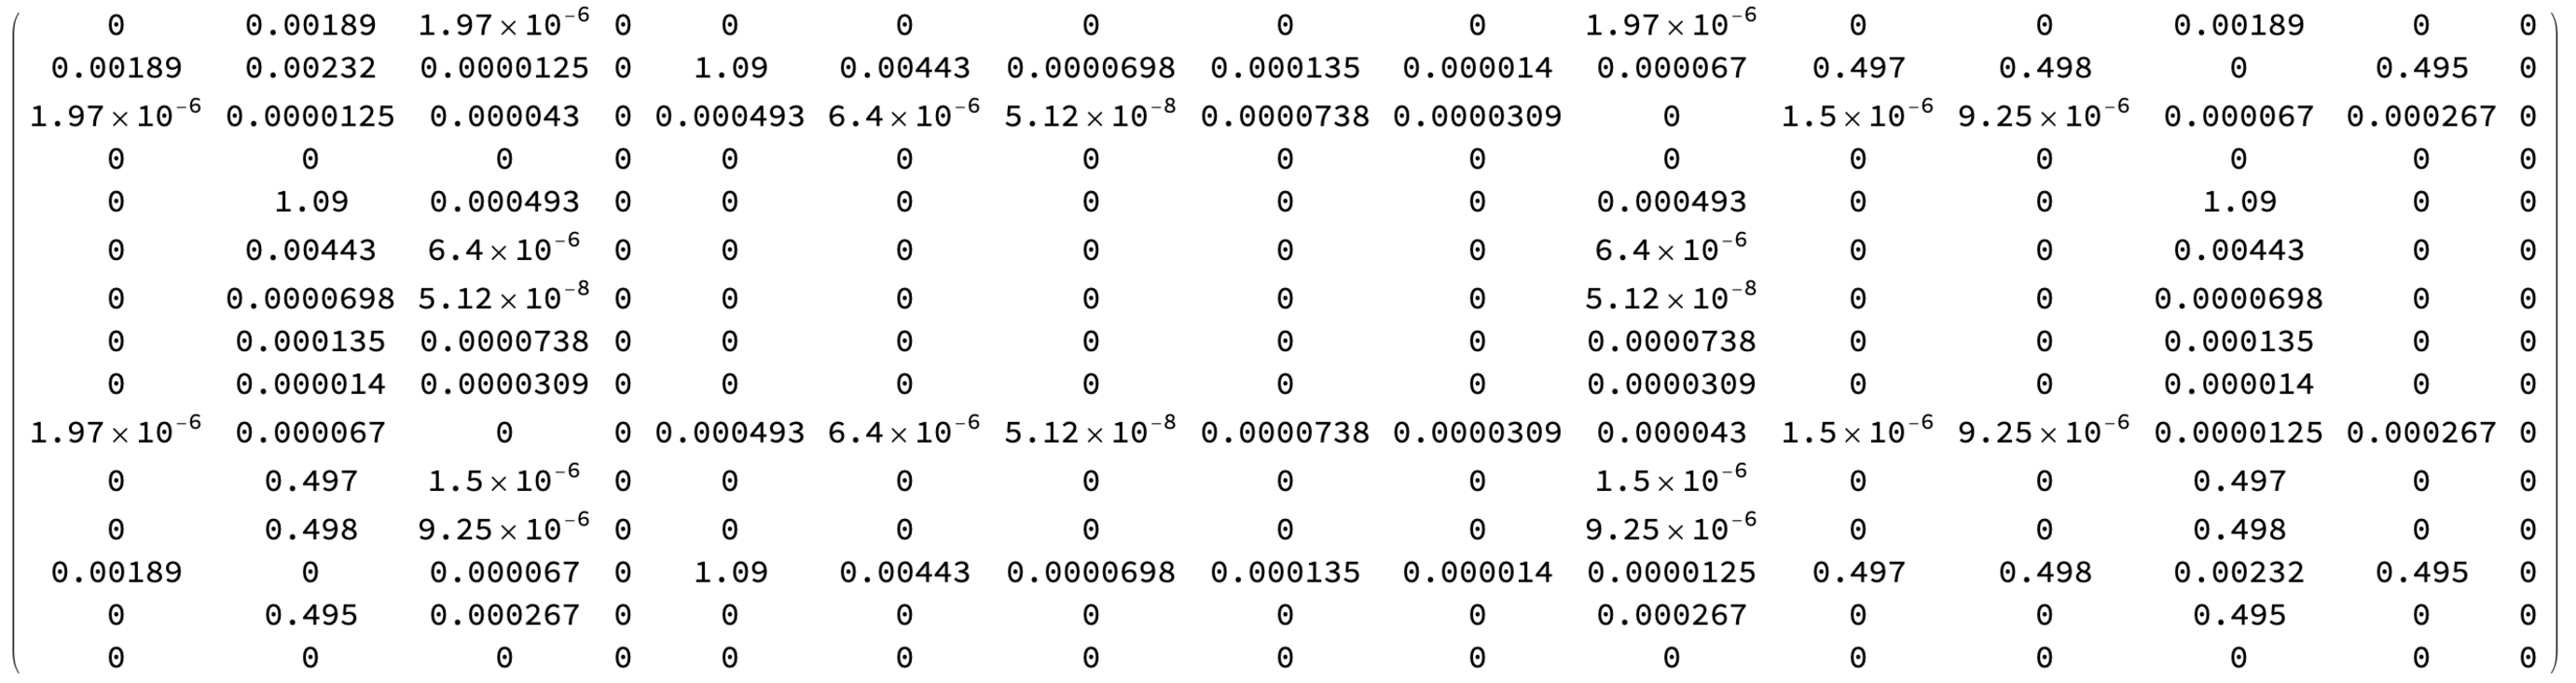
\includegraphics[width=1\textwidth]{Error_lu.pdf}
    \caption{Error between the matrix inverses (LU decomposition).}
    \label{fig:lu_inverse_error}
\end{figure}

Firstly, the pivot could be found in any position of the matrix. However, the error between the inverses yields relatively high values, as depicted in Fig. \ref{fig:lu_inverse_error}. Seeking to reduce the error, LU decomposition is performed again, but now only pivoting diagonal elements is allowed. Figures \ref{fig:lu_L_diag} - \ref{fig:lu_inverse_error_diag} show the results for the decomposition.
\begin{figure}[H]
    \centering
    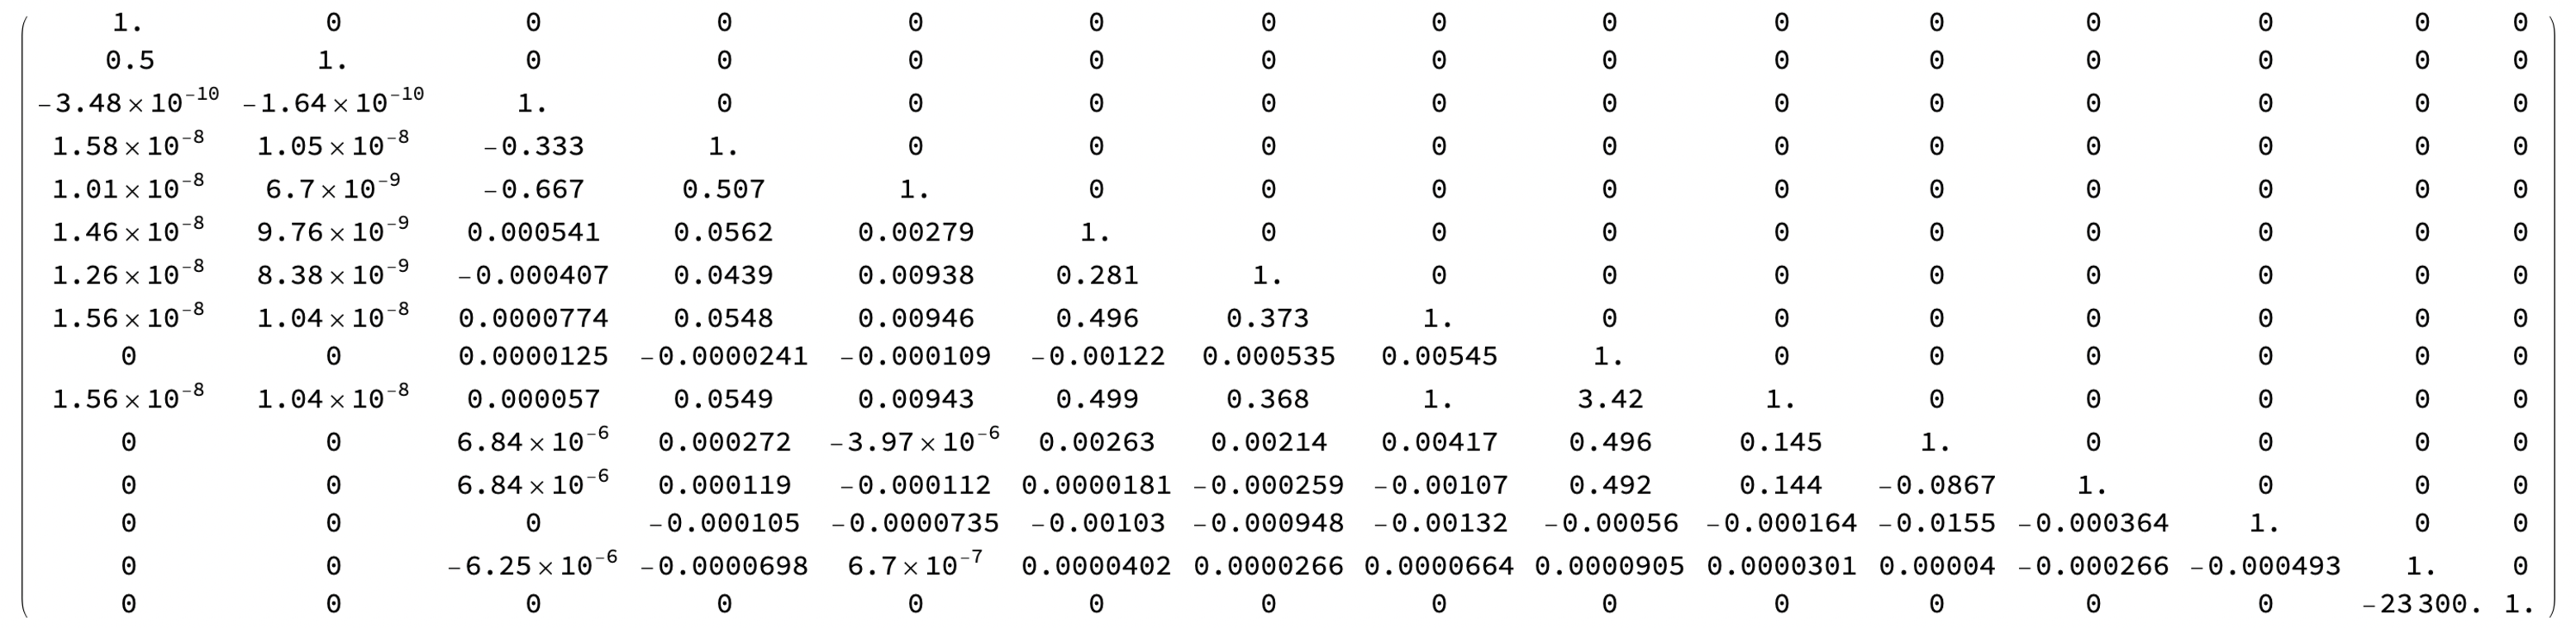
\includegraphics[width=1\textwidth]{L_lu_diag.pdf}
    \caption{Matrix L (LU diagonal pivoting decomposition).}
    \label{fig:lu_L_diag}
\end{figure}
\begin{figure}[H]
    \centering
    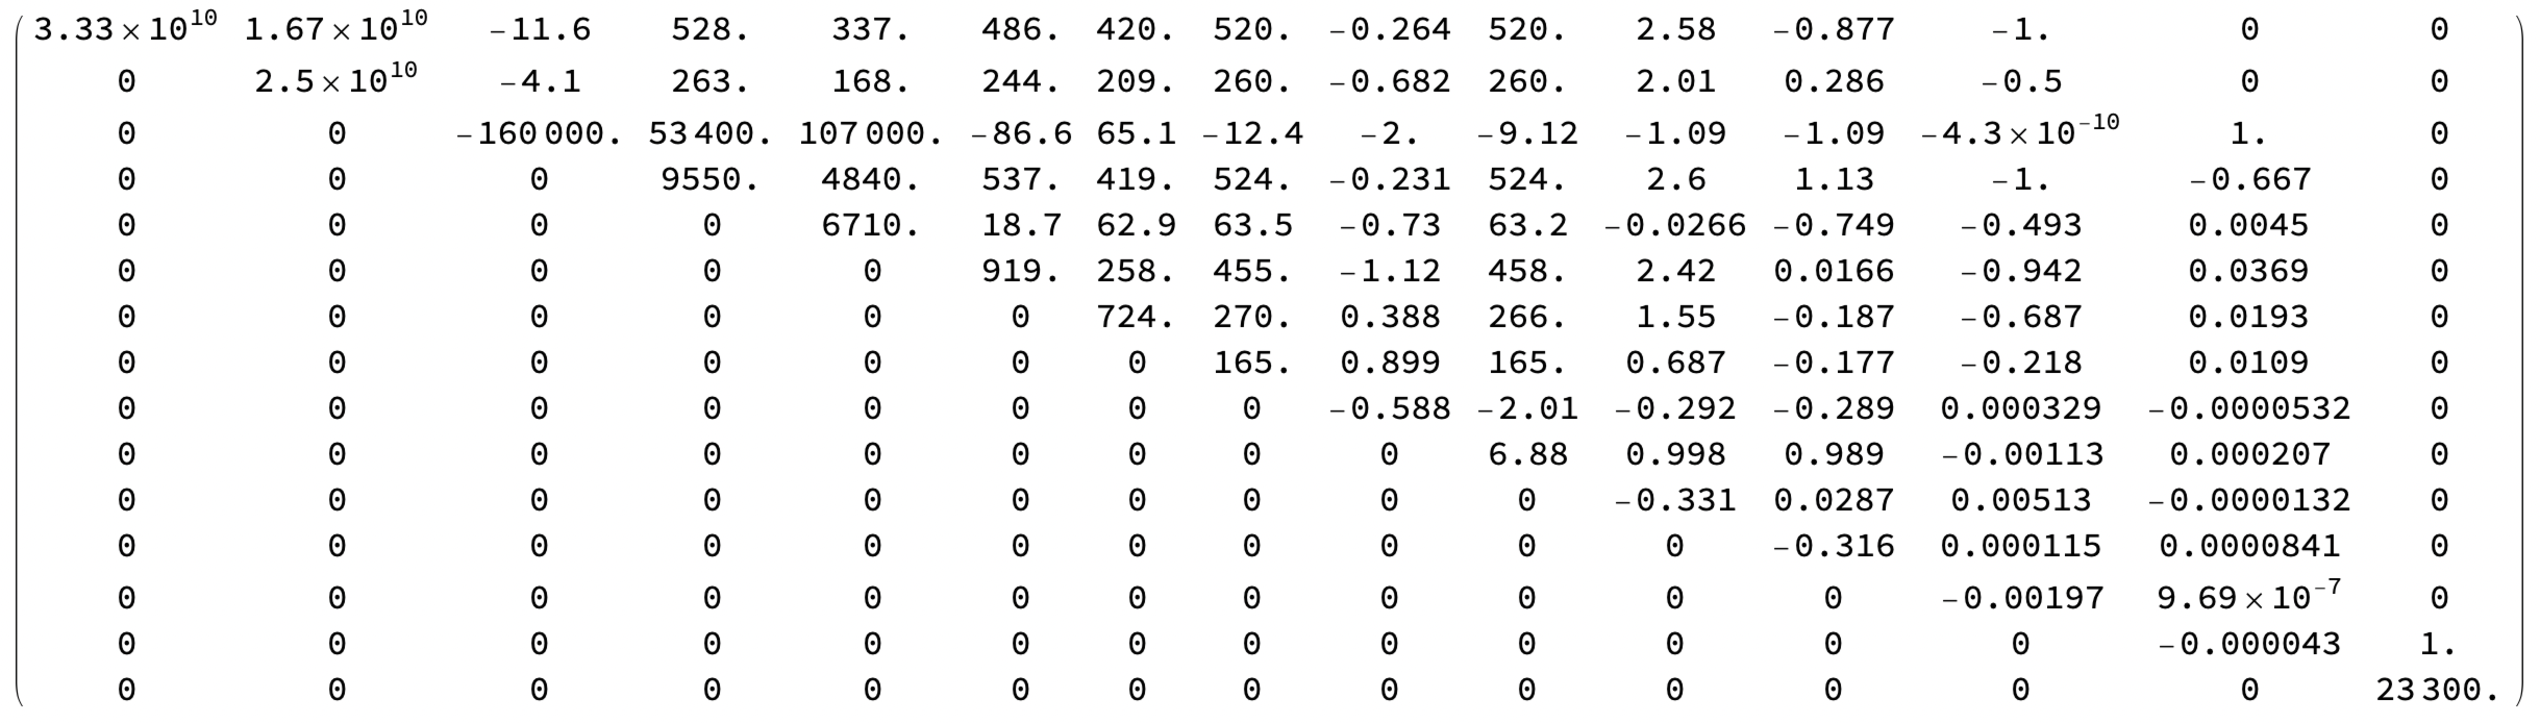
\includegraphics[width=1\textwidth]{U_lu_diag.pdf}
    \caption{Matrix U (LU diagonal pivoting decomposition).}
    \label{fig:lu_inverse_error_diag}
\end{figure}
\begin{figure}[H]
    \centering
    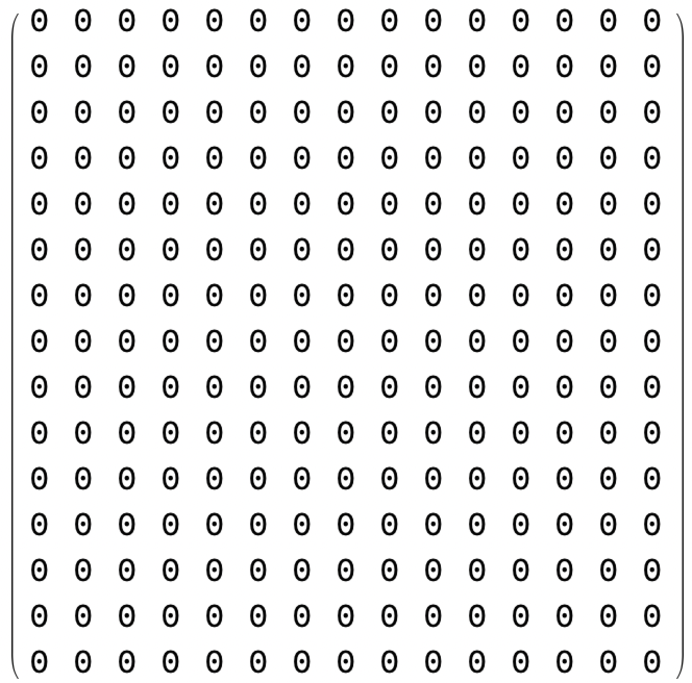
\includegraphics[width=.5\textwidth]{Error_lu_diag.pdf}
    \caption{Error between the matrix inverses (LU diagonal pivoting decomposition).}
    \label{fig:lu_inverse_error_diag}
\end{figure}

A quick comparison between both decompositions shows that matrices L and U pivoting any element have residuals that do not appear when only diagonal elements are pivoted. Results for pivoting only the diagonal elements seem to be more accurate for this matrix, as the error between the inverses is smaller. Notice that the error matrice is processed by Mathematica using the Chop filter, which sets to zero any value below a certain threshold.

Appendix \ref{sec:PermutationMatrices} shows the permutation matrices for both LU decompositions. 

\subsection{Matrix LDLt Decomposition} \label{sec:ldlt}
Results for matrices L, D and U are depicted in figures \ref{fig:ldlt_L} - \ref{fig:ldlt_U}. T
\begin{figure}[H]
    \centering
    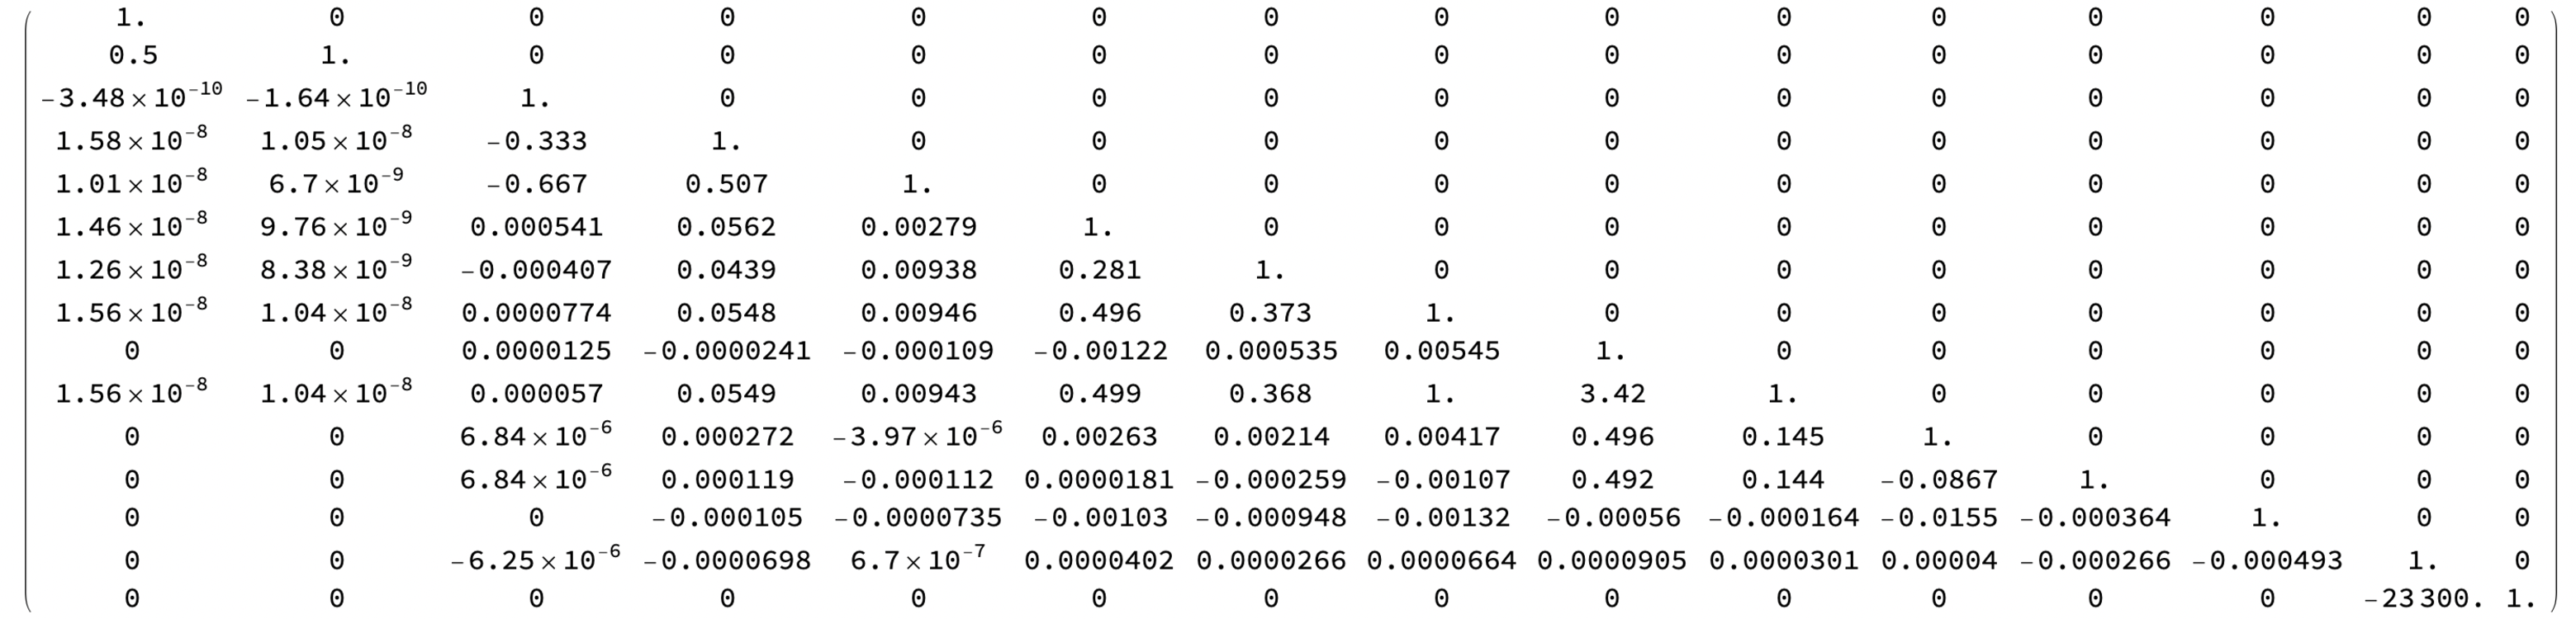
\includegraphics[width=1\textwidth]{L_ldlt.pdf}
    \caption{Matrix L (LDLt decomposition).}
    \label{fig:ldlt_L}
\end{figure}
\begin{figure}[H]
    \centering
    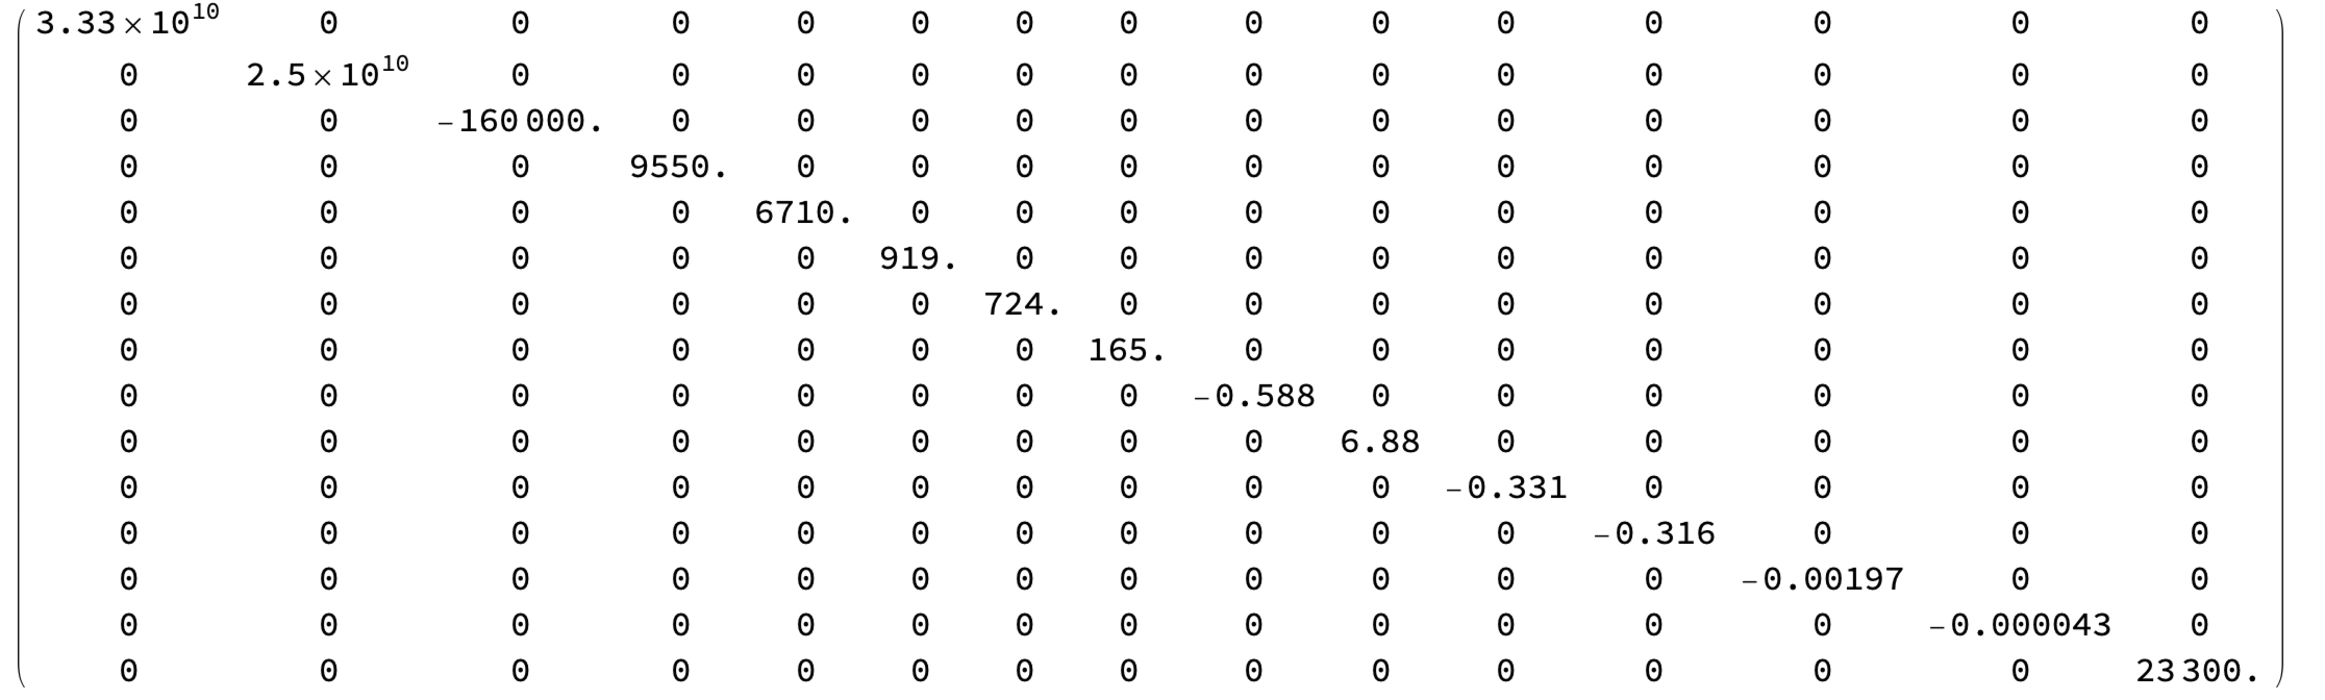
\includegraphics[width=1\textwidth]{D_ldlt.pdf}
    \caption{Matrix D (LDLt decomposition).}
    \label{fig:ldlt_D}
\end{figure}
\begin{figure}[H]
    \centering
    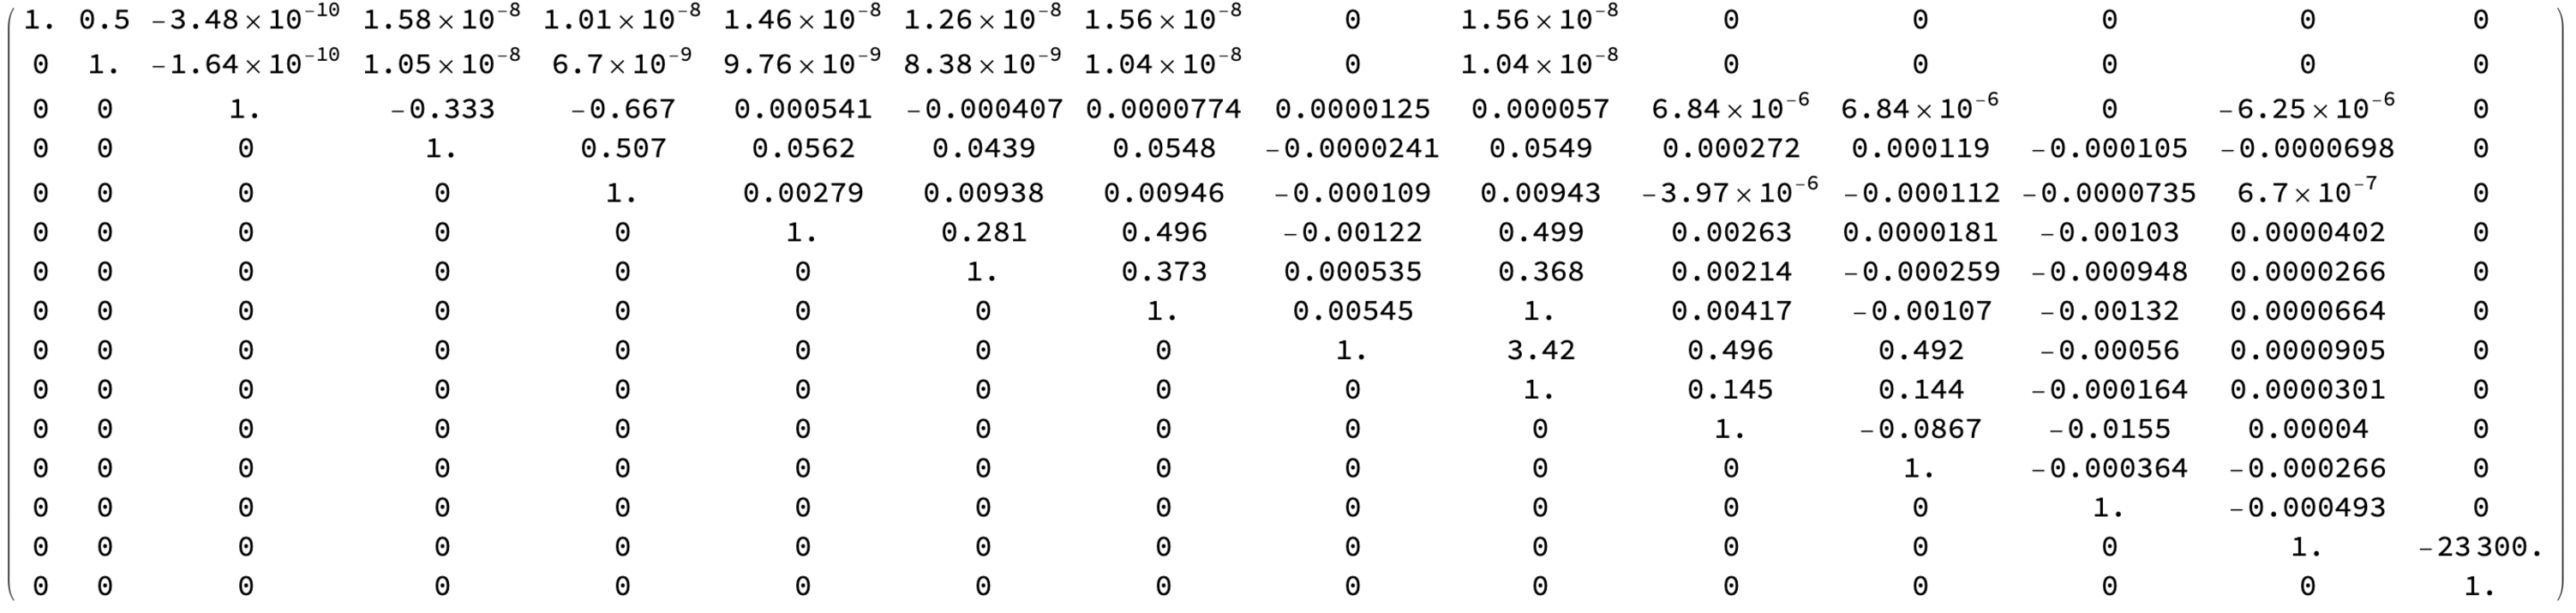
\includegraphics[width=1\textwidth]{U_ldlt.pdf}
    \caption{Matrix U (LDLt decomposition).}
    \label{fig:ldlt_U}
\end{figure}

The error between the original matrix inverse and the decomposed matrix inverse is shown in Fig. \ref{fig:ldlt_inverse_error}.Appendix \ref{sec:PermutationMatrices} shows the permutation matrices for the LDLt decomposition.
\begin{figure}[H]
    \centering
    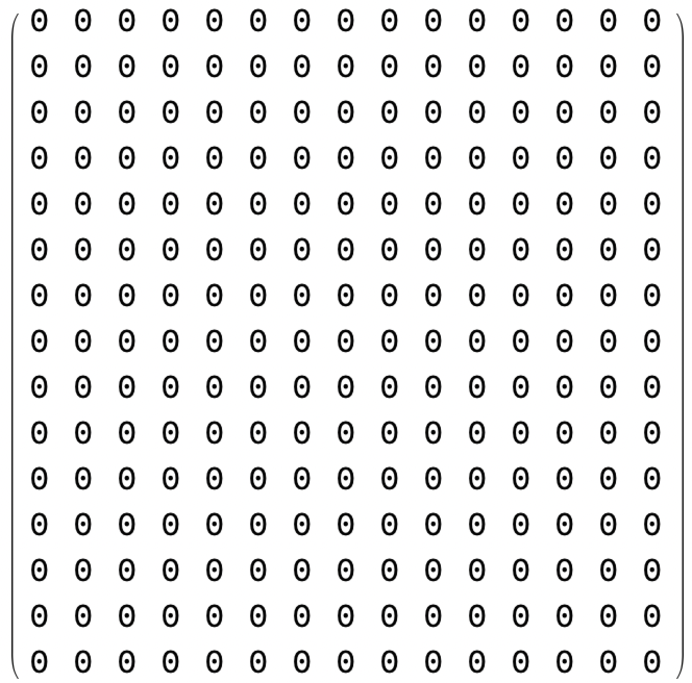
\includegraphics[width=.5\textwidth]{Error_ldlt.pdf}
    \caption{Error between the matrix inverses (LDLt decomposition).}
    \label{fig:ldlt_inverse_error}
\end{figure}

As a way to compare the methods, Table \ref{tab:error} shows the norm of the error between the inverse matrices in each decomposition. The norm of the error is calculated as the sum of the absolute values of the difference between the inverse matrices. 
\begin{table}[H]
    \centering 
    \caption{Error between the inverse matrices.}
    \begin{tabular}{cc}
        \hline
        Decomposition & Error \\
        \hline
        LU & 2.77 \\ 
        LU (Diagonal Pivoting) & 5.72e-13 \\
        LDLt & 6.30e-13 \\ \hline
    \end{tabular}
    \label{tab:error}
\end{table}

One understands that the error is smaller for LU decomposition with diagonal pivoting, followed by LDLt decomposition. However, since the values are near to machine precision, numerical errors might influence the results.
\section{The Sparse Matrix Class}\label{sec:sparsematrix}

\subsection{Class Implementation} \label{sec:sparsematrix_implementation}

\subsection{Storage Structure and Memory Usage} \label{sec:storage}

\subsection{Product Matrix Vector} \label{sec:product}
\section{Conclusions} \label{sec:conclusions}
This work implemented two classes: FullMatrix and SparseMatrix. FullMatrix has LU and LDLt decomposition methods for solving linear systems, which after analyses it was observed that LU decomposition with diagonal pivoting has resulted in the smallest errors in terms of inverse recovery, followed by LDLt decomposition. 

When it comes to sparse matrices, it is observed that the decision whether to use it or not is based on a series of factors, such as the sparsity of the matrix, the number of non-zero elements, and the size of the matrix. Not always sparse matrices result in less memory usage. 

Finally, the process of operating a sparse matrix is not trivial, and the algorithm must be adapted to this structure. Otherwise, several errors may arise during the code's execution and more necessary than the necessary might be allocated to finish the process. 

% ------- BIBLIOGRAPHY -------
\addcontentsline{toc}{section}{References}
\bibliographystyle{abntex2-num}
\bibliography{References}

% ------- APPENDIX -------
\appendix
\section{GitHub Repository}\label{sec:github}
 The source code for this report and every code inhere mentioned can be found in the following GitHub repository: \href{https://github.com/CarlosPuga14/MetodosNumericos_2024S1}{CarlosPuga14/MetodosNumericos\_2024S1}.

\end{document}